\documentclass[]{article}
\usepackage{amssymb}
\usepackage{amsmath}
\usepackage[utf8]{inputenc}
\usepackage{graphicx}
\usepackage{booktabs}
\usepackage{listings}
\usepackage{color}
\usepackage{tabularx}
\usepackage{hyperref}

\definecolor{dkgreen}{rgb}{0,0.6,0}
\definecolor{gray}{rgb}{0.5,0.5,0.5}
\definecolor{mauve}{rgb}{0.58,0,0.82}

\lstset{frame=tb,
	%language=C++,
	aboveskip=3mm,
	belowskip=3mm,
	showstringspaces=false,
	columns=flexible,
	basicstyle={\small\ttfamily},
	numbers=none,
	numberstyle=\tiny\color{gray},
	keywordstyle=\color{blue},
	commentstyle=\color{dkgreen},
	stringstyle=\color{mauve},
	breaklines=false,
	breakatwhitespace=true,
	tabsize=2
}


\title{FYS-STK4155 H20 - Project 2:\\Neural nets}
\author{Olav Fønstelien}

\begin{document}
\maketitle

\begin{abstract}
%The abstract gives the reader a quick overview of what has been done and the most important results. Try to be to the point and state your main findings. It could be structured as follows 
% - Short introduction to topic and why its important 
% - Introduce a challenge or unresolved issue with the topic (that you will try to solve) 
% - What have you done to solve this 
% - Main Results 
% - The implications

\end{abstract}

\section{Introduction} \label{intro}
%When you write the introduction you could focus on the following aspects
% - Motivate the reader, the first part of the introduction gives always a motivation and tries to give the overarching ideas
% - What I have done
% - The structure of the report, how it is organized etc

% Refer to project 1 and the inefficiency and limitations of linear regression -> SGD + logistic regression -> limits of logistic regression -> neural networks
In \cite{project1} we studied linear regression methods. We saw that for the Ordinary Least Squares (OLS) and Ridge methods we had to calculate a matrix product on the form $(\mathbf{X}^\intercal \mathbf{X} + \lambda \mathbf{I})^{-1} \mathbf{X}^\intercal$ in order to obtain the coefficient estimates $\mathbf{\hat{\beta}}$ ($\lambda = 0$ for OLS). As we saw, the matrix inversion operation may be numerically unstable, and if we need a large number of samples to approximate the function, this operation becomes computationally demanding or even infeasible. 

The Stochastic Gradient Descent method (SGD) deals with both of these problems. It still requires calculating $\mathbf{X}^\intercal \mathbf{X}$, but since it determines the coefficient estimates $\mathbf{\hat{\beta}}$ iteratively on so-called \textit{mini batches} which can be kept in the higher levels of cache, the operation becomes less computationally demanding. The inversion operation is avoided all-together. 

SGD is useful in other methods as well. SGD can be used in logistic regression methods, which lets us solve \textit{classification problems} where we predict the outcome of an event as the one most likely of several possible \textit{classes} of outcomes. For these problems, linear regression methods are unsuitable. Logistic regression again is unsuitable for the class of problems where the decision boundary between features and outcomes is non-linear, like the \textit{XOR} (exclusive or) logical operator. For these problems, Artificial Neural Networks (ANNs) can be used.

In this report we will ....





\clearpage
\section{Methods} \label{methods}
% - Describe the methods and algorithms
% - You need to explain how you implemented the methods and also say something about the structure of your algorithm and present some parts of your code
% - You should plug in some calculations to demonstrate your code, such as selected runs used to validate and verify your results. The latter is extremely important!! A reader needs to understand that your code reproduces selected benchmarks and reproduces previous results, either numerical and/or well-known closed form expressions.

In this section we will develop methods for solving regression and classification problems with traditional linear and logistic regression methods, as well as Feed-Forward Neural Network, a simple type of ANN. In the outline I will use matrix notation where possible, since this closely resembles the implementation in a computer programming environment with array programming capabilities like native MATLAB, C++ with the \lstinline|armadillo| lib or Python with the \lstinline|numpy| module, which I will use.

\subsection{Stochastic Gradient Descent}
Stochastic Gradient Descent is a numerical method for minimizing the cost function of a mathematical optimization method like OLS or logistic regression, where the minimization is done in an iterative, stochastic approach on a selection of the full set of samples. That is; given a cost function $\mathcal{C}(\mathbf{\beta})$, where $\mathbf{\beta} \in \mathbb{R}^p$, SGD lets us solve the problem
\begin{equation}
	\frac{\partial \mathcal{C}(\mathbf{\beta})}{\partial \mathbf{\beta}} = \mathbf{0},
\end{equation}
where a closed-form solution is otherwise not available, or computationally expensive, and by using only a sub-set of the samples in each iteration. It is based on the iterative application of Newton-Raphson's method on the coefficient vector $\mathbf{\beta}$, such that
\begin{equation} \label{newton-raphson}
	\mathbf{\beta}^{(i+1)} = \mathbf{\beta}^{(n)} - [\mathbf{H}^{(i)}]^{-1}\mathbf{g}^{(i)},
\end{equation}
where $\mathbf{g}$ is the gradient of the cost function and $\mathbf{H}$ is its Hessian matrix, each given by
\begin{equation}
	\mathbf{g}^{(i)} = \frac{\partial \mathcal{C}(\mathbf{\beta}^{(i)})}{\partial \mathbf{\beta}} \quad \text{, and} \quad 
	\mathbf{H}^{(i)} = \frac{\partial^2 \mathcal{C}(\mathbf{\beta}^{(i)})}{\partial \mathbf{\beta} \partial \mathbf{\beta}^\intercal}.
\end{equation}
Equation (\ref{newton-raphson}) can be deduced from the Taylor expansion of $\mathcal{C}(\mathbf{\beta})$ around $\mathbf{\beta}^{(i+1)} - \mathbf{\beta}^{(i)}$. See \cite{fys-stk4155-notes} for a thorough outline of this.

Calculating the Hessian and inverting it is an expensive and numerically volatile operation, so our approach will be to replace it by a scalar $\eta$, the so-called \textit{learing rate}, such that $\mathbf{H}^{-1} \rightarrow \eta$. Equation (\ref{newton-raphson}) thus becomes
\begin{equation} \label{newton-raphson-eta}
	\mathbf{\beta}^{(i+1)} = \mathbf{\beta}^{(i)} - \eta \mathbf{g}^{(i)}.
\end{equation}

Finding the \textit{best} $\eta = \hat{\eta}$, such that $\mathbf{\beta}^{(i+1)} = \mathbf{\hat{\beta}}$ again involves calculating the Hessian, unfortunately \cite{fys-stk4155-notes}; 
\begin{equation}
	\hat{\eta} = \frac{\mathbf{g}^\intercal \mathbf{g}}{\mathbf{g}^\intercal \mathbf{H} \mathbf{g}}.
\end{equation}
However, the cost function $\mathcal{C}(\mathbf{\beta})$ is guaranteed to be convex for linear and logistic regression problems, implying a positive definite $\mathbf{H}$ \cite{murphy2012machine}. Therefore, as long as we select $\eta < 2/\lambda_{max}$, where $\lambda_{max}$ is the largest eigenvalue of the Hessian matrix, Equation (\ref{newton-raphson-eta}) will converge towards $\mathbf{\hat{\beta}}$. Again, $\lambda_{max}$ will remain unknown to us; but knowing that if we select a $\eta$ which is not too large, a solution will be found, we base our approach on trial and error. 

\vspace{5mm}

The next problem then becomes to decide when to stop the search for $\mathbf{\hat{\beta}}$. One solution is to stop when the difference between the iterations becomes smaller than some defined value, $||\mathbf{\beta}^{(n+1)} - \mathbf{\beta}^{(n)}||_2 \le \varepsilon$. Another, which we will use here, is simply to define a number of iterations, and extract the solution thereafter. This might seem a little inaccurate, maybe, but works well since the direction of $\mathbf{g}$ is always towards the global minimum, and $|\mathbf{g}| \rightarrow 0$ when $\mathbf{\beta} \rightarrow \mathbf{\hat{\beta}}$, which means that if we come close to $\mathbf{\hat{\beta}}$, the final approximation $\mathbf{\beta}^{(final)} \approx \mathbf{\hat{\beta}}$.

A further refinement to this is to incrementally decrease $\eta$ for each iteration towards $\mathbf{\hat{\beta}}$; that is to let $\eta \rightarrow \eta^{(i)} = f(i)$, such that $\eta^{(i+1)} < \eta^{(i)}$. This increases the stability of the method since it allows us to even have $\eta^{(0)} > 2/\lambda_{max}$ and still get convergence.

Two such \textit{learning schedules} $\eta^{(i)} = f(i)$ are the \lstinline|invscaling| schedule in Python's \lstinline|scikit-learn| module \cite{skl};
\begin{equation} \label{invscaling}
	\eta^{(i)} = \frac{\eta^{(0)}}{i^k},
\end{equation}
and another one suggested by Geron in \cite{geron2019hands};
\begin{equation} \label{geron}
	\eta^{(i)} = \frac{t_0}{i + t_1}.
\end{equation}
Here the factors $k, t_0, t_1$ are user defined. Figure \ref{fig:learning_schedules} shows each learning schedule with some selections for the user-defined factors over the 100 first iterations.

\vspace{5mm}

Calculating the gradient of the cost function $\mathbf{g}$ in Equation (\ref{newton-raphson-eta}) may prove computationally demanding if the data set is large. The gradient of the logistic regression method cost function, for instance, would require that we calculate the matrix product $\mathbf{X}^\intercal \mathbf{P}$ in each iteration. In SGD, we select a subset of the samples by a stochastic process, and calculated an approximated gradient based on this subset or mini batch. The standard deviation of the gradient's expectation value relative to the number of samples $n$ follows the relation \cite{fys-stk4155-notes}
\begin{equation}
	\sigma_g \sim \frac{1}{\sqrt{n}},
\end{equation}
which means that if we collect a mini batch of 100 from a data set of 1000 samples, the standard deviation will only increase by a factor of 3, but the computation of each iteration will run 10 times faster.

Another great advantage of only approximating the gradient on a mini sample is the decreased risk of getting stuck in a local minimum or saddle point, where $\mathbf{g} \rightarrow 0$, but $\mathbf{\beta} \neq \mathbf{\hat{\beta}}$. This is especially useful in neural network applications, where it is not given that we have a convex cost function.

The implementation of SGD is outlined in Listing \ref{lst:sgd}. An \lstinline|epoch| is defined as a full run through the full set of samples. The \lstinline|learning_schedule()|s could be as in Equations (\ref{invscaling}) and (\ref{geron}). 

\vspace{5mm}

The \lstinline|cost_function_gradient()|s that we will use in this report are Mean Squared Error (MSE), used in OLS and Ridge regression methods; and Cross Entropy (CE), used in the logistic regression method. MSE cost function gradient is given by
\begin{equation} \label{cost-mse}
	\mathbf{g}_{mse}^{(n)} = \frac{\partial \mathcal{C}_{mse}^{(n)}}{\partial \mathbf{\beta}} = \frac{1}{n} (\mathbf{X}^\intercal \mathbf{X}) \mathbf{\beta}^{(n)} - \mathbf{X}^\intercal \mathbf{y} + \lambda \mathbf{\beta}^{(n)},
\end{equation}
where $\mathbf{y}$ is the response variable vector and $\lambda$ is the $L_2$ regularization parameter \cite{project1}. 

The CE cost function gradient is given by
\begin{equation} \label{cost-mse}
	\mathbf{g}_{ce}^{(n)} = \frac{\partial \mathcal{C}_{ce}^{(n)}}{\partial \mathbf{\beta}} = \frac{1}{n} (\mathbf{X}^\intercal \mathbf{P}^{(n)} - \mathbf{X}^\intercal \mathbf{Y}) + \lambda \mathbf{\beta}^{(n)}.
\end{equation}
Here, $\mathbf{Y} \in \mathbb{R}^{n \times c}$ is the response variable matrix with $n$ samples and $c$ different classes of outcome. Each row $\mathbf{y}_i$ has a single 1, and the rest 0s. Likewise, $\mathbf{P} \in \mathbb{R}^{n \times c}$ is the probability matrix for the $n$ samples and $c$ classes following the \textit{softmax} function:
\begin{equation}
	\mathbf{P} = \mathrm{softmax}(\mathbf{X}'\mathbf{B}).
\end{equation}
$\mathbf{X}'$ is the design matrix with an intercept column added in front $\mathbf{X}' = [\mathbf{1} \quad \mathbf{X}]$. The coefficient matrix $\mathbf{B} \in \mathbb{R}^{(p+1) \times c}$, accounting for the intercept, i.e. the variation in outcomes not explained by the features in $\mathbf{X}$. $\mathbf{B}$ is given by
\begin{equation}
	\mathbf{B} = [\mathbf{\beta}_1 \quad \mathbf{\beta}_2 \quad \cdots \quad \mathbf{\beta}_c], \quad \text{where} \quad \mathbf{\beta}_j = [\beta_{0j} \quad \beta_{1j} \quad \cdots \quad \beta_{pj}]^\intercal.
\end{equation}

Each element $p_{ij}$ in $\mathbf{P}$ is given by
\begin{equation} \label{log-reg-pij}
	p_{ij} = \mathrm{softmax}(\mathbf{X}'\mathbf{B})_{ij} = \frac{\mathrm{exp}(\mathbf{x}_i'\mathbf{\beta}_j)} {\sum_{c}\mathrm{exp}(\mathbf{x}_i'\mathbf{\beta}_c)},
\end{equation}
and the sum of each row $\mathbf{p}_i$ in $\mathbf{P}$ is 1; $\sum_{j} p_{ij} = 1$.

\vspace{5mm}

In Figure \ref{fig:demo_lin_log_reg} we see a demonstration on some mock-up cases for each of the regression methods OLS and Rdge with SGD, and logistic with SGD. For the linear regression cases, a simple linear function with some noise has been used; $y_i = 1 + 2x_i + \varepsilon_i$, where $\mathbf{\epsilon} \sim \mathcal{N}(0, 0.75^2)$, and samples $n=100$. We see that both methods make the fit quite well after 20 epochs and 10 mini batches with constant learning schedule with $\eta = 0.5$ for OLS and $\eta = 0.7, \lambda=0.1$ for Ridge.

The logistic regression classification problem mock-up is shown in Table \ref{tab:logreg-demo}. The design matrix $\mathbf{X}'$ is generated by adding some noise to an identity matrix of dimension $3 \times 3$, and adding the intercepts. Each of the three cases represent distinct outcomes, $\mathbf{Y}$. To the right in Figure \ref{fig:demo_lin_log_reg} we see that when we use the result of the logistic regression $\mathbf{B}$ to fit to $\mathbf{X}'$, correct outcomes are predicted with high confidence in each case.

\begin{figure}[!htb]
	\centering
	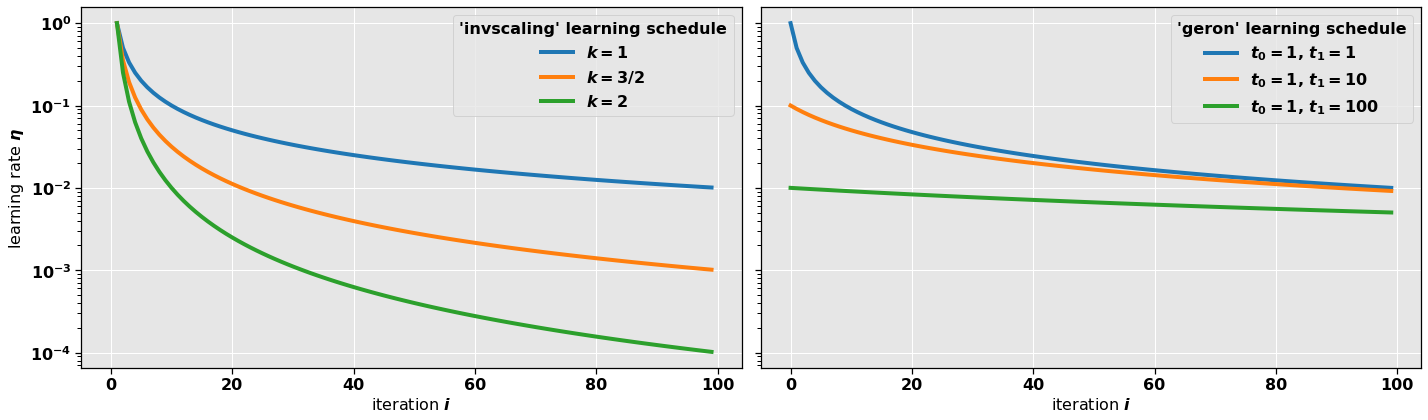
\includegraphics[width=1\linewidth]{learning_schedules.png}
	\caption{Two different learning schedules over the 100 first iterations. To the left we see the \lstinline|invscaling| schedule in Python's \lstinline|scikit-learn| module, as given in Equation (\ref{invscaling}). To the right we see the simple schedule suggested by Geron, as given in Equation (\ref{geron}).}
	\label{fig:learning_schedules}
\end{figure}

\begin{figure}[!htb]
	\centering
	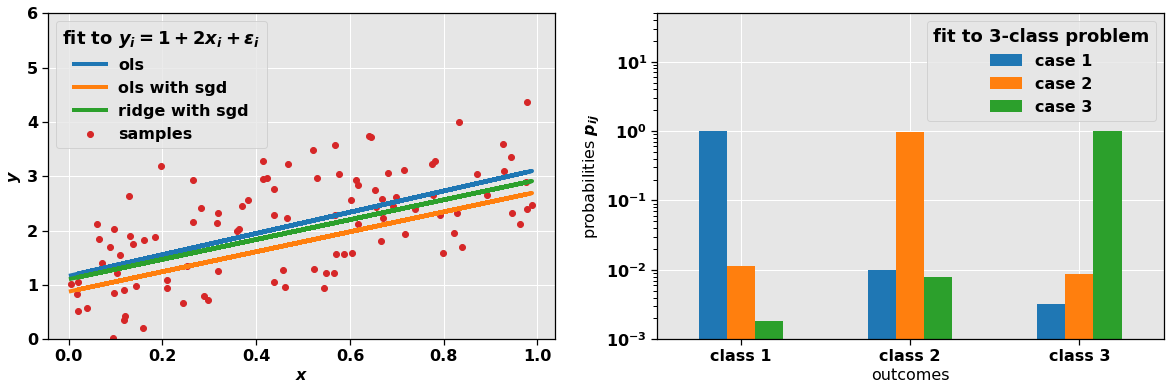
\includegraphics[width=1\linewidth]{demo_lin_log_reg.png}
	\caption{Demonstration of linear regression to the left, and logistic regression to the right using the SGD method. For linear regression, the fit is guaranteed to be best for the simple OLS case since the model we try to fit corresponds exactly to to the function which generated the samples, but we see that both OLS with SGD and Ridge with SGD approach simple OLS. For logistic regression, a mock-up model of a $3 \times 3$ design matrix $\mathbf{X}$ plus intercept is fitted to a $3 \times 3$ one-hot matrix $\mathbf{Y} = \mathbf{I}$. See Table \ref{tab:logreg-demo}. To generate the result, $\mathbf{X}$ has been fed into the softmax function together with the result of the regression fit $\mathbf{B}$ (Equation (\ref{log-reg-pij})). We see that we pick the right class with high confidence in each case.}
	\label{fig:demo_lin_log_reg}
\end{figure}

\begin{minipage}{\linewidth}
	\begin{lstlisting}[caption={Stochastic Gradient Descent algorithm. Cost function gradients and learning schedules may be defined independently of the implementation of SGD. This implementation runs for \lstinline|epochs*batches| iterations, and does not sense if or when it converges.},label={lst:sgd}] [!ht]
		// Declarations
		betas = "initial coefficient values"
		epochs = "number of runs through data set"
		batches = "number of mini batches"
		iteration_number = 0
		
		// Inputs
		data = "the design matrix"
		targets = "the response variables"
	
		// SGD process	
		FOR i = 1...epochs DO
			shuffle(data, targets)
			FOR j = 1...batches DO
				data_batch, targets_batch = "draw mini batch from full set w/o replacement"
				iteration_number++
				eta = learning_schedule(iteration_number, args...)
				grad = cost_function_gradient(data_batch, targets_batch)
				betas = betas - eta*grad
			END FOR
		END FOR
	\end{lstlisting}
\end{minipage}

\begin{table}[!ht]
	\caption{Mock-up classification problem for demonstration of logistic regression. The table has three cases or samples 1,2,3, which are represented with the design matrix $\mathbf{X}'$ in the middle and the one-hot response variable matrix $\mathbf{Y}$ to the right. See the result of the demo to the right in Figure \ref{fig:demo_lin_log_reg}.}
	\label{tab:logreg-demo}
	\begin{center}
		\begin{tabular}{r|rrrr|rrr}
			\toprule
			case &  intercept &     $p_1$ &     $p_2$ &     $p_3$ &  class 1 &  class 2 &  class 3 \\
			\midrule
			1 &          1 &  1.548814 &  0.715189 &  0.602763 &        1 &        0 &        0 \\
			2 &          1 &  0.544883 &  1.423655 &  0.645894 &        0 &        1 &        0 \\
			3 &          1 &  0.437587 &  0.891773 &  1.963663 &        0 &        0 &        1 \\
			\bottomrule
		\end{tabular}
	\end{center}
\end{table}


\subsection{Feed-Forward Neural Network}
The linear and logistic regression methods each have their well-defined set of problems where they come to use; regression and classification, respectively. Artificial Neural Networks is another method, which is can be used for both types of problems, including classification problems with non-linear decision boundaries, like the XOR logical operator, or binary number representation. In this report we study a type of ANN called Feed-Forward Neural Network (FFNN).

Figure \ref{fig:ann-illustration} gives an illustration of a typical FFNN. The layers consist of one or more \textit{nodes} with a \textit{activation function}. Each node-to-node connection has a \textit{weight}, and the input to each node's activation function is the weighted sum of the inputs from all the nodes in the former layer, plus a node-specific \textit{bias}. Except for in the input layer, where the design matrix $\mathbf{X}$ is fed in, all the activation functions are non-linear. This gives the network a highly non-linear behavior. The output of the first hidden layer is thus a non-linear transformation of the information in the input layer, and this process is repeated in the succeeding layers, including the output. At the output layer, the output is evaluated against a suitable cost function, and the error is back-propagated up through the network, which regulates the incremental update of weights and biases. This \textit{training} process is then repeated for a given number of times, or until we have convergence.

\vspace{5mm}

What follows now is a mathematical derivation of the feed-forward, back-propagation and variable update of an FFNN. It is in large part based on \cite{fys-stk4155-notes}, but translated into full matrix notation for simpler implementation in an array programming environment. The reader is encouraged to refer to this source for a thorough, general outline.

As indicated above, the input layer in our FFNN does not have an activation function, it only passes the design matrix $\mathbf{X}$ on to the first hidden layer. If we let $\mathbf{X} \in \mathbb{R}^{n \times p}$, the input layer will have $p$ nodes which are all connected to the $m$ nodes of layer 1, the first hidden layer. Layer 1's weight matrix $\mathbf{W}_1 \in \mathbb{R}^{p \times m}$ is then given as
\begin{equation}
	\mathbf{W}_1 = 
	\left[\begin{array}{cccc}
		w_{11} &w_{12} & \cdots &w_{1m} \\
		w_{21} &w_{22} & \cdots &w_{2m} \\
		\vdots &\vdots &\vdots  &\vdots \\ 
		w_{p1} &w_{p2} & \cdots &w_{pm} \\
	\end{array} \right]_{(1)},
\end{equation} 
and its biases are
\begin{equation}
	\mathbf{b}_1 = [b_1 \quad b_2 \quad \cdots \quad b_m]_{(1)}.
\end{equation}
The resulting inputs $\mathbf{Z}_1$ to layer 1's activation function $f_1$ then become
\begin{equation} \label{inputs}
	\mathbf{Z}_1 = \mathbf{X} \mathbf{W}_1 + \mathbf{B}_1, \quad \text{where} \quad \mathbf{Z}_1, \mathbf{B}_1 \in \mathbb{R}^{n \times m}.
\end{equation}
Here, $\mathbf{B}_1$ is the bias matrix; an $n \times m$ matrix with $\mathbf{b}_1 \in \mathbb{R}^m$ repeated in all its $n$ rows.

Layer 1's activation function output $\mathbf{A}_1$ is given by
\begin{equation} \label{outputs}
	\mathbf{A}_1 = f_1(\mathbf{Z}_1) \in \mathbb{R}^{n \times m},
\end{equation}
which is fed into the preceding layer, where this process is repeated. Here we note that this output $\mathbf{A}_1$ is a non-linear transformation of the input $\mathbf{X}$ to the network, which is true also for the remaining layers, including the output layer.

\vspace{5mm}

Let $L$ denote the output layer in our FFNN and $\cal{C}(\mathbf{\theta})$ the cost function of out model, where $\mathbf{\theta}$ may be any variable which influences its value. We evaluate the output of our FFNN against this cost function and update the output layer's weights and biases according to the gradient of the cost function with respect to each set of variables $\mathbf{W}_L, \mathbf{b}_L$;
\begin{equation} \label{wb-update}
\begin{aligned}
		\mathbf{W}_L &\leftarrow \mathbf{W}_L - \eta \frac{\partial \mathcal{C}}{\partial \mathbf{W}_L} \\
		\mathbf{b}_L &\leftarrow \mathbf{b}_L - \eta \frac{\partial \mathcal{C}}{\partial \mathbf{b}_L} \\
\end{aligned},
\end{equation}
where $\eta$ is the learning rate, a hyperparameter.

By the chain rule, it can be shown that
\begin{equation} \label{hadamard}
\begin{aligned}
	\frac{\partial \mathcal{C}}{\partial \mathbf{W}_L} &= 
	\mathbf{A}_{L-1}^\intercal \left(\frac{\partial \mathcal{C}}{\partial \mathbf{A}_L} \circ \frac{df_L}{d\mathbf{Z}_L} \right) \\
	\frac{\partial \mathcal{C}}{\partial \mathbf{b}_L} &= 
	\frac{\partial \mathcal{C}}{\partial \mathbf{A}_L} \circ \frac{df_L}{d\mathbf{Z}_L} \\
\end{aligned},
\end{equation}
where $\circ$ denotes the element-wise Hadamard product. Here we will let $\mathbf{\Delta}_L$ denote this Hadamard product or error term in Equation (\ref{hadamard});
\begin{equation} \label{delta-L}
	\mathbf{\Delta}_L = \frac{\partial \mathcal{C}}{\partial \mathbf{A}_L} \circ \frac{df_L}{d\mathbf{Z}_L}.
\end{equation}
Equation (\ref{wb-update}) now becomes
\begin{equation}
\begin{aligned}
	\mathbf{W}_L &\leftarrow \mathbf{W}_L - \eta \mathbf{A}_{L-1}^\intercal \mathbf{\Delta}_L \\
	\mathbf{b}_L &\leftarrow \mathbf{b}_L - \eta \mathbf{\Delta}_L \\
\end{aligned}.
\end{equation}

The preceding layers up to but not including the input are then updated in a similar fashion by back-propagation of this error up through the network. Again by the chain rule, it can be shown that $\mathbf{\Delta}_{L-1}$ is given by
\begin{equation}
	\mathbf{\Delta}_{L-1} = (\mathbf{\Delta}_L \mathbf{W}_L^\intercal) \circ \frac{df_{L-1}}{d\mathbf{Z}_{L-1}}.
\end{equation}
For the general layer $l \ge 1$, $\mathbf{\Delta}_l$ becomes
\begin{equation} \label{update-deltas}
	\mathbf{\Delta}_{l} = (\mathbf{\Delta}_{l+1} \mathbf{W}_{l+1}^\intercal) \circ \frac{df_l}{d\mathbf{Z}_l},
\end{equation}
and the rule for updating layer $l$'s weights and biases becomes
\begin{equation} \label{update-weights-biases}
\begin{aligned}
	\mathbf{W}_l &\leftarrow (1 - \eta \lambda) \mathbf{W}_l - \eta \mathbf{A}_{l-1}^\intercal \mathbf{\Delta}_l \\
	\mathbf{b}_l &\leftarrow \mathbf{b}_l - \eta \mathbf{\Delta}_l \\
\end{aligned}.
\end{equation}
Here, we have added $\lambda$, the $L_2$ regularization parameter, which follows by the cost function derivation with respect to $\mathbf{W}_L$;
\begin{equation}
	\mathcal{C}' = \mathcal{C} + \frac{\lambda}{2} ||\mathbf{W}_L||_2^2 \rightarrow \frac{\partial \mathcal{C}'}{\partial \mathbf{W}_L} = \frac{\partial \mathcal{C}}{\partial \mathbf{W}_L} + \lambda \mathbf{W}_L.
\end{equation}

\vspace{5mm}

Like for the Stochastic Gradient Descent method discussed in the previous section, the ANN training process is then repeated until convergence, when $||\mathcal{C}(\mathbf{\theta})||_2 \le \varepsilon$, or for a defined number of times, which we will do in this report.

\vspace{5mm}

Neural networks are generally data hungry \cite{fys-stk4155-notes}, so to make the ANN training process as efficient as possible, we will use the Stochastic Gradient Descent method here as well. Another advantage of this approach is that the scattered descent reduces the chance of having the learning process getting stuck in local minima or saddle points. This only involves putting the training process inside the double epochs-batches loop in Listing \ref{lst:sgd}. An outline of the training process is given in Listing \ref{lst:ann-training}.

\vspace{5mm}

The \lstinline|activation_function()|s and \lstinline|activation function_derivative()|s in Listing \ref{lst:ann-training} are very simple non-linear functions. Many types and variants for each type exist, but in this project we limit ourselves to those listed in Table \ref{tab:activation-funcs}.

%, with shapes as shown in Figure XX.

The \lstinline|cost_function_derivative()|s in Listing \ref{lst:ann-training} which we will use in this report are the derivatives with respect to the outputs $\mathbf{A}_L$ of the Mean Squared Error cost function (MSE) and the Cross Entropy cost function (CE). The MSE derivative is given by
\begin{equation}
	\frac{\partial \mathcal{C}_{mse}}{\partial \mathbf{A}_L} = (\mathbf{A}_L - \mathbf{Y}),
\end{equation}
and the CE derivative by
\begin{equation} \label{ce-partial}
	\frac{\partial \mathcal{C}_{ce}}{\partial a_L^{(ij)}} = \frac{a_L^{(ij)} - y^{(ij)}}{a_L^{(ij)} (a_L^{(ij)} - y^{(ij)})}.
\end{equation}
Equation (\ref{ce-partial}) is due to \cite{fys-stk4155-notes}.

\vspace{5mm}

Figure \ref{fig:demo_lin_log_ffnn} shows the simple mock-up regression and classification problems used for SGD demonstration in the previous chapter (Figure \ref{fig:demo_lin_log_reg}) solved by our FFNN.

For the regression problem we fit a network with 1 hidden layer. It has 2 nodes in the input and hidden layers, and 1 node in the output. The activation function is always sigmoid, and the cost function MSE. We have trained this network on $n = 100$ samples $y_i = 1 + 2x_i + \varepsilon_i$ for 100 epochs with mini batches of 10 samples and use $\eta = 0.5$ and the constant training schedule. The 100 samples are then fed back in to make a prediction. We see that as expected the prediction is a non-linear curve, and that it closely follows the OLS fit, but with a slight bend.

Classification is done on the 3-class problem described in Table \ref{tab:logreg-demo}. Again the FFNN has 1 hidden layer, but with 4 nodes in the input and hidden layers, and 3 nodes in the output layer. The hidden layer activation function is ReLU, and the output layer function is softmax, which is suitable for multiclass problems. The cost function is Cross Entropy. We have trained the network for 100 epochs with batch size 1, $\eta = 0.1$ and $L_2$ regularization $\lambda = 0.001$. In the input data cases 1,2,3 correspond to classes 1,2,3, which is also the prediction of our FFNN when the training data is fed back into the network for testing.

\begin{figure}[!htb]
	\centering
	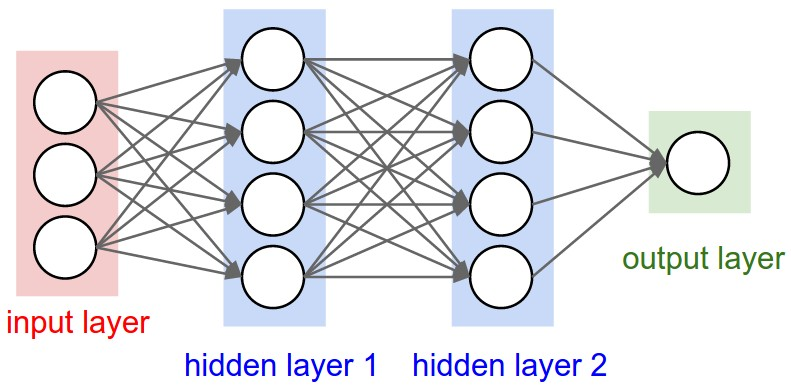
\includegraphics[width=1\linewidth]{ann-illustration.jpeg}
	\caption{ANN with one input layer, two hidden layers, and an output layer. The design matrix is fed into the input layer, and is fed through the hidden layers and the output layer value is evaluated against a cost function. The error is then back-propagated and regulates the adjustment of the weights associated with each node-to-node connection and the bias of each node are in order to make a better fit in the next iteration. To introduce non-linearity, the output of each node is decided by the inputs and bias fed into a non-linear activation function. This network could be used for either regression, or binary classification. Illustration borrowed from \cite{fys-stk4155-notes}.}
	\label{fig:ann-illustration}
\end{figure}

\begin{figure}[!htb]
	\centering
	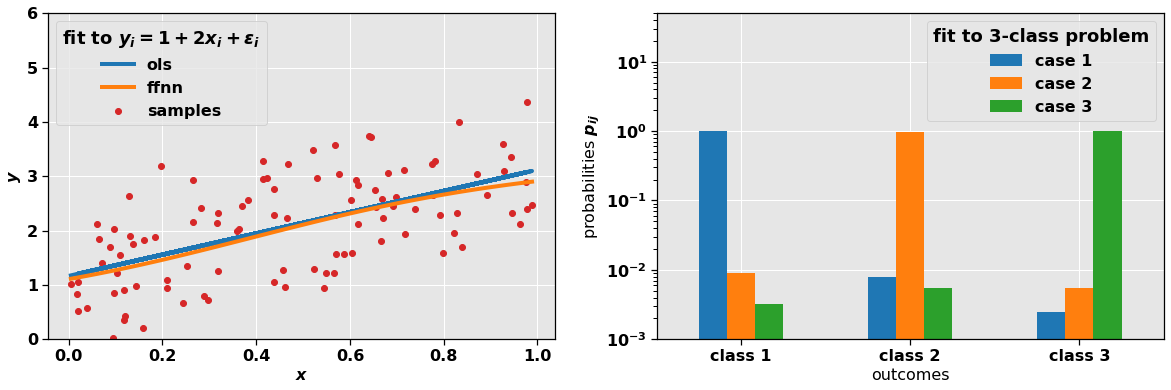
\includegraphics[width=1\linewidth]{demo_lin_log_ffnn.png}
	\caption{Demonstration of FFNN on a simple regression problem to the left, and a simple classification problem to the right. For linear regression, the fit is guaranteed to be best for the simple OLS case since the model we try to fit corresponds exactly to to the function which generated the samples, but we see that the FFNN finds a non-linear fit which closely follows the OLS line. For the classification problem, we predict three cases with three features and three classes of outcome. In the input data cases 1,2,3 correspond to classes 1,2,3, respectively. See Table \ref{tab:logreg-demo} for details. We see that we pick the right class with high confidence in each case. Compare with Figure \ref{fig:demo_lin_log_reg}, which shows the same set of problems solved by linear and logistic regression methods.}
	\label{fig:demo_lin_log_ffnn}
\end{figure}

%\begin{minipage}{\linewidth}
	\begin{lstlisting}[caption={Outline of the Feed-Forward Neural Network training process using a Stochastic Gradient Descent scheme. The weights and biases in each layer must be initiated with some value.},label={lst:ann-training},escapeinside={@}{@}] [!t]
	// Declarations
	layers = "collection of layers in the FFNN"
	epochs = "number of runs through data set"
	batches = "number of mini batches"
	iteration_number = 0
	lmd = "L2 regularization parameter"
	
	// Inputs
	data = "the design matrix"
	targets = "the response variables"
	
	// SGD learning process
	FOR i = 1...epochs DO
		shuffle(data, targets)
		FOR j = 1...batches DO
			data_batch, targets_batch = "draw mini batch from full set w/o replacement"
			
			// Feed forward
			layer_outputs = data_batch			
			FOR EACH layer IN layers DO
				"set layer's inputs by @Equation (\ref{inputs})@"
				"set layer's outputs by activation_function() @Equation (\ref{outputs})@"
			END FOR EACH
			
			// Calculate the cost function derivative with respect to output
			// layer outputs and targets
			error = cost_function_derivative("output layer's output", targets_batch)
			
			// Back-propagate the error by @Equations (\ref{delta-L}) and (\ref{update-deltas})@
			FOR EACH layer IN REVERSED(layers) DO
				"set layer's activation function_derivative() with respect to its inputs"
				"set layer's deltas by the back-propagated error"
				error = "error to back-propagate by this layer's new delta and weights"
			END FOR EACH		
			
			// Update weigths and biases
			iteration_number++
			eta = learning_schedule(iteration_number, args...)
			FOR EACH layer IN layers DO
				"update layer's weights by @Equation (\ref{update-weights-biases})@ with step eta, reg. lmd"
				"update layer's biases by @Equation (\ref{update-weights-biases})@ with step eta"
			END FOR EACH
		END FOR
	END FOR
	\end{lstlisting}
%\end{minipage}


\begin{table}[!ht]
	\caption{Various activation functions and their derivatives. More variants and types exist, but these are the ones used in this report. ReLU, leaky-ReLU and unit-step derivatives are not defined at $z=0$, but we approximate them as 0 here. Also, the derivative of unit-step is of course always 0, but to progress the learning process it is defined as shown here. The unit-step is usually best suited for classification problems, and softmax especially for multiclass problems. For linear regression problems, sigmoid or one of the ReLUs can be used.}
	\label{tab:activation-funcs}
	\begin{center}
		\begin{tabular}{l|l|l|l}
			\toprule
			name&	$f(z)$&	$f'(z)$&	asymptote \\
			\midrule
			ReLU&	$\mathrm{max}(0,z)$&	1 if $z > 0$; 0 else&	$0,+\infty$ \\
			leaky-ReLU&	$\mathrm{max}(0.01z,z)$&	1 if $z > 0$; 0.01 else&	$-\infty,+\infty$ \\
			unit-step&	1 if $z > 0$; 0 else&	set to 1 if $z > 0$; 0 else&	$0,+1$ \\
			sigmoid&	$1/(1 + e^{-z})$&	$\mathrm{sigmoid}(z)(1 - \mathrm{sigmoid}(z))$	&	$0,+1$ \\
			softmax&	$e^{z_{ij}}/\sum_{c}e^{z_{ic}}$&	$\mathrm{softmax}(z_{ij})(1 - \mathrm{softmax}(z_{ij}))$ &	$0,+1$ \\
			\bottomrule
		\end{tabular}
	\end{center}
\end{table}


\clearpage
\section{Results} \label{results}
% - Present your results
% - Give a critical discussion of your work and place it in the correct context.
% - Relate your work to other calculations/studies
% - An eventual reader should be able to reproduce your calculations if she/he wants to do so. All input variables should be properly explained.
% - Make sure that figures and tables should contain enough information in their captions, axis labels etc so that an eventual reader can gain a first impression of your work by studying figures and tables only.

\subsection{Stochastic Gradient Descent: Linear Regression}
%Perform an analysis of the results for OLS and Ridge regression as function of the chosen learning rates, the number of mini-batches and epochs as well as algorithm for scaling the learning rate.

\subsection{Stochastic Gradient Descent: Logistic Regression}
%Study the results as functions of the chosen learning rates. Add also an l2 regularization parameter λ. Compare your results with those from your FFNN code as well as those obtained using Scikit-Learn's logistic regression functionality. 

\subsection{Feed-Forward Neural Network: Regression}
%Train your network and compare the results with those from your OLS and Ridge Regression codes from project 1. You should test your results against a similar code using Scikit-Learn

%Comment your results and give a critical discussion of the results obtained with the Linear Regression code and your own Neural Network code. Compare the results with those from project 1. Make an analysis of the regularization parameters and the learning rates employed to find the optimal MSE and R2 scores.

%You should now also test different activation functions for the hidden layers. Try out the Sigmoid, the RELU and the Leaky RELU functions and discuss your results. You may also study the way you initialize your weights and biases. 

\subsection{Feed-Forward Neural Network: Classification}
%We will here study the MNIST data set of hand-written numbers. Use the Softmax function as activation function. Your code should however also be able to use a binary activation function as well. 

%Discuss your results and give a critical analysis of the various parameters, including hyper-parameters like the learning rates and the regularization parameter λ (as you did in Ridge Regression), various activation functions, number of hidden layers and nodes and activation functions. 


\clearpage
\section{Discussion and Conclusion} \label{conclusion}
% - State your main findings and interpretations
% - Try as far as possible to present perspectives for future work
% - Try to discuss the pros and cons of the methods and possible improvements

\clearpage
\bibliographystyle{unsrt}
\bibliography{project2.bib}
\end{document}
